\begin{frame}{Motivation}
  \begin{itemize}
    \item Traditional NLP models are \textbf{unimodal} (text-only) and \textbf{reactive}.
    \item Modern AI agents need to perceive, reason, and act in complex environments using \textbf{multiple modalities} (e.g., vision, text, speech).
    \item \textbf{Multimodal systems} and \textbf{agentic AI} aim to build goal-directed, autonomous, and continuously learning agents.
    \item Rise of agent frameworks (Auto-GPT, BabyAGI) and vision-language models enables new research frontiers in decision-making, robotics, and assistive AI.
  \end{itemize}
\end{frame}

\begin{frame}{What is multimodality?}
  \begin{columns}[T,onlytextwidth]
    \column{0.62\textwidth}
      \vspace{-1ex}
      {\Large\bfseries multimodal \textit{adjective}}

      \vspace{0.3em}
      \textipa{[m\ae lt\textlengthmark \textturna\textquotedblleft m\textturna\textlengthmark d\textschwa l]}
      
      \vspace{0.4em}
      : having or involving several modes, modalities, or maxima

      \vspace{0.18em}
      \textit{multimodal distributions}

      \textit{multimodal therapy}
      
      \vspace{1.2em}
      {\small
      In our case, focusing on NLP: text + one or more other \textit{modality} (images, speech, audio, olfaction, others). We'll mostly focus on images as the other modality.
      }

    \column{0.34\textwidth}
      \centering
      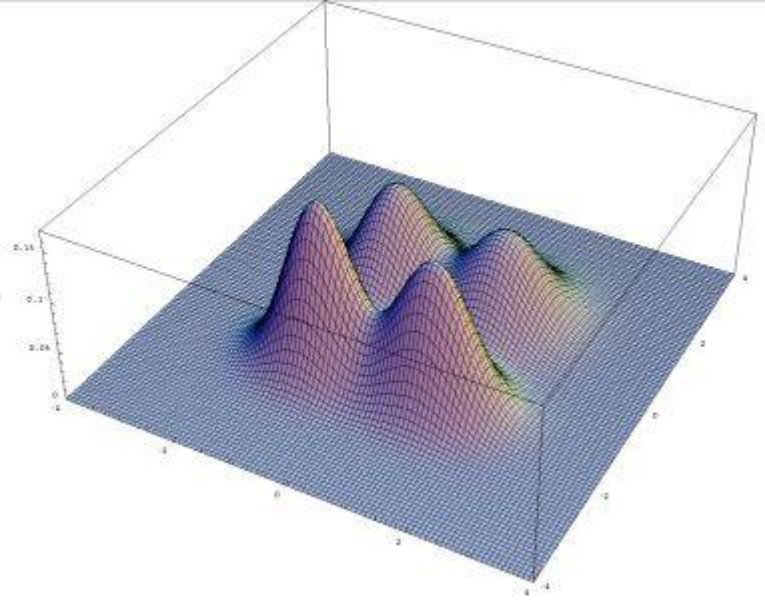
\includegraphics[width=0.7\textwidth, height=0.7\textheight, keepaspectratio]{assets/Lecture-10_Multimodal_NLP_Agentic_AI/slide_006.png}
  \end{columns}
\end{frame}

\begin{frame}{Multimodal brains}
  \begin{itemize}
    \item \textbf{McGurk effect} (McGurk \& MacDonald, 1976)
      \begin{itemize}
        \item Classic demonstration of interaction between modalities (audio + vision) in perception
        \item Speech sound is misheard depending on visual (lip movement) cues
      \end{itemize}
    \item \href{https://www.youtube.com/watch?v=2k8fHR9jKVM}{Watch this demonstration on YouTube}
  \end{itemize}
  \vspace{1em}
  \centering
  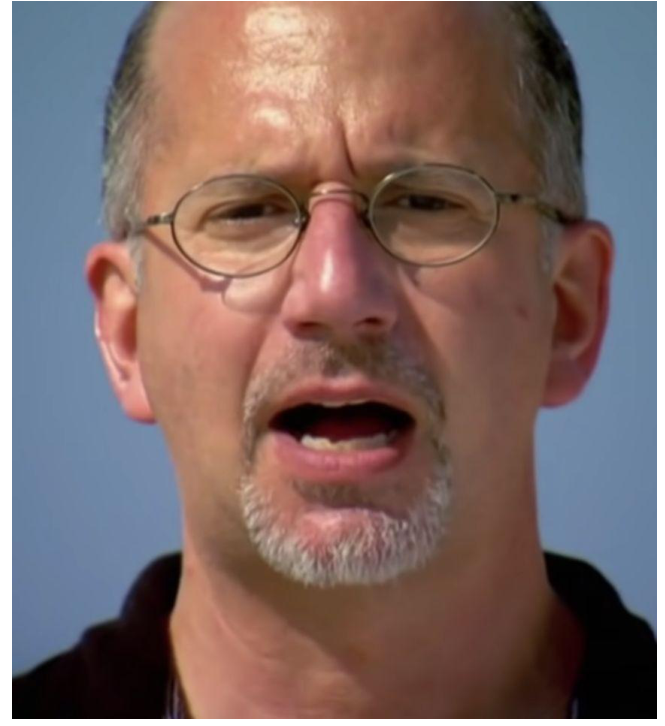
\includegraphics[width=0.50\textwidth, height=0.50\textheight, keepaspectratio]{assets/Lecture-10_Multimodal_NLP_Agentic_AI/slide_007.png}
\end{frame}
